% =============================================================================
%  pic-tex/example-tikz/example-tikz-source.tex
%  STANDALONE TikZ source of the example figure.
%  Compile this file by itself to produce example-tikz-source.pdf:
%      cd pic-tex/example-tikz
%      xelatex example-tikz-source.tex
%  The resulting PDF is included by example-tikz.tex (the figure wrapper).
%
%  This is the recommended workflow for all figures: keep a standalone TikZ
%  source per figure, compile it to PDF, and include the PDF in the paper.
%  图片工作流：每个图保留一个独立的 TikZ 源文件，单独编译为 PDF 后插入正文。
% =============================================================================

\documentclass[border=8pt]{standalone}

\usepackage{tikz}
\usetikzlibrary{calc,positioning}
\definecolor{winered}{rgb}{0.5,0,0}   % match main.tex link color

\begin{document}

% REPLACE with your own figure. This is a placeholder showing a stylized
% time series of "ruler power security" across three periods.
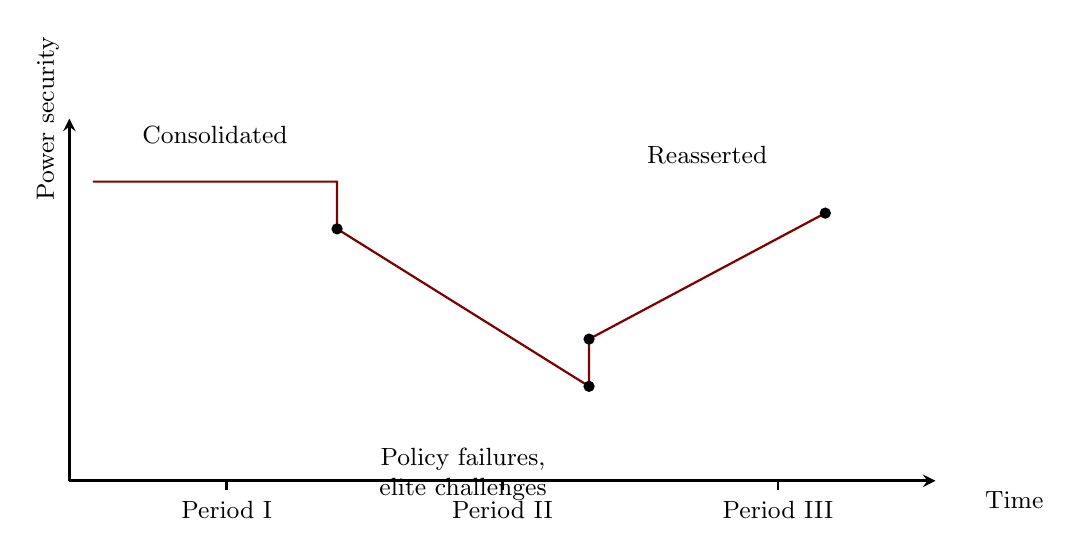
\begin{tikzpicture}[
    font=\small,
    >=stealth,
    line width=1pt
  ]
  % axes
  \draw[->] (0,0) -- (11,0) node[below, xshift=1cm] {Time};
  \draw[->] (0,0) -- (0,4.6) node[above, rotate=90, anchor=south] {Power security};

  % tick labels
  \foreach \x/\lab in {2/Period I, 5.5/Period II, 9/Period III}
    \draw (\x,0) -- (\x,-0.12) node[below] {\lab};

  % step function: high -> low -> high
  \draw[winered, thick]
    (0.3,3.8) -- (3.4,3.8) -- (3.4,3.2)
    (3.4,3.2) -- (6.6,1.2) -- (6.6,1.8)
    (6.6,1.8) -- (9.6,3.4);

  % annotations
  \node[align=center, above] at (1.85,4.15) {Consolidated};
  \node[align=center, below] at (5.0,0.55) {Policy failures, \\ elite challenges};
  \node[align=center, above] at (8.1,3.9) {Reasserted};

  % dummy data points (placeholder)
  \filldraw (3.4,3.2) circle (1.5pt);
  \filldraw (6.6,1.2) circle (1.5pt);
  \filldraw (6.6,1.8) circle (1.5pt);
  \filldraw (9.6,3.4) circle (1.5pt);
\end{tikzpicture}

\end{document}
